%
% The first command in your LaTeX source must be the \documentclass command.
\documentclass[sigconf]{acmart}

%
% defining the \BibTeX command - from Oren Patashnik's original BibTeX documentation.
\def\BibTeX{{\rm B\kern-.05em{\sc i\kern-.025em b}\kern-.08emT\kern-.1667em\lower.7ex\hbox{E}\kern-.125emX}}
    
% Rights management information. 
% This information is sent to you when you complete the rights form.
% These commands have SAMPLE values in them; it is your responsibility as an author to replace
% the commands and values with those provided to you when you complete the rights form.
%
% These commands are for a PROCEEDINGS abstract or paper.
\copyrightyear{2019} 
\acmYear{2019} 
\setcopyright{acmcopyright}
\acmConference[ITiCSE '19]{Innovation and Technology in Computer Science Education}{July 15--17, 2019}{Aberdeen, Scotland, UK}
\acmBooktitle{Innovation and Technology in Computer Science Education (ITiCSE '19), July 15--17, 2019, Aberdeen, Scotland, UK}
\acmPrice{15.00}
\acmDOI{10.1145/3304221.3319776}
\acmISBN{978-1-4503-6301-3/19/07}

\settopmatter{printacmref=true}
\fancyhead{}

%
% These commands are for a JOURNAL article.
%\setcopyright{acmcopyright}
%\acmJournal{TOG}
%\acmYear{2018}\acmVolume{37}\acmNumber{4}\acmArticle{111}\acmMonth{8}
%\acmDOI{10.1145/1122445.1122456}

%
% Submission ID. 
% Use this when submitting an article to a sponsored event. You'll receive a unique submission ID from the organizers
% of the event, and this ID should be used as the parameter to this command.
%\acmSubmissionID{123-A56-BU3}

%
% The majority of ACM publications use numbered citations and references. If you are preparing content for an event
% sponsored by ACM SIGGRAPH, you must use the "author year" style of citations and references. Uncommenting
% the next command will enable that style.
%\citestyle{acmauthoryear}

%
% end of the preamble, start of the body of the document source.
\begin{document}

%
% The "title" command has an optional parameter, allowing the author to define a "short title" to be used in page headers.
\title{Pedagogical Content for Professors of Introductory Programming Courses}

%
% The "author" command and its associated commands are used to define the authors and their affiliations.
% Of note is the shared affiliation of the first two authors, and the "authornote" and "authornotemark" commands
% used to denote shared contribution to the research.
\author{Yorah Bosse}
\authornote{The first author is financially supported by the UFMS - Federal University of Mato Grosso do Sul.}
%\orcid{1234-5678-9012}
\affiliation{%
  \institution{University of Sao Paulo / Federal University of Mato Grosso do Sul }
%  \streetaddress{Sao Paulo / Ponta Pora}
  \city{Sao Paulo / Ponta Pora}
  \country{Brazil}
%  \postcode{43017-6221}
}
\email{yorah@ime.usp.br}

\author{David Redmiles}
%\authornote{DFR information.}
\affiliation{%
  \institution{University of California}
%  \streetaddress{P.O. Box 1212}
  \city{Irvine}
  \country{USA}
%  \postcode{43017-6221}
}
\email{redmiles@ics.uci.edu}

\author{Marco A. Gerosa}
%\authornote{MAG information.}
\affiliation{%
  \institution{Northern Arizona University / University of Sao Paulo}
%  \streetaddress{1 Th{\o}rv{\"a}ld Circle}
  \city{Flagstaff / Sao Paulo}
  \country{USA / Brazil}}
\email{marco.gerosa@nau.edu}

%
% By default, the full list of authors will be used in the page headers. Often, this list is too long, and will overlap
% other information printed in the page headers. This command allows the author to define a more concise list
% of authors' names for this purpose.
\renewcommand{\shortauthors}{Y. Bosse, et al.}

%
% The abstract is a short summary of the work to be presented in the article.
\begin{abstract}
Teaching introductory programming requires knowledge of both content and pedagogy. Pedagogy includes understanding the typical difficulties students face as they learn, as well as recognizing didactic strategies professors can use to help students to overcome these difficulties. Our research aims to improve the pedagogical knowledge instructors have to teach introductory programming courses, especially those new in this area. We conducted 16 semi-structured interviews with instructors who teach introductory programming courses and collected diaries filled by 110 students during their studies. Qualitative analysis of this data revealed a set of difficulties students faced when learning programming basics and a set of didactic strategies professors use to mitigate them. The results were reviewed by senior instructors in order to confirm them and by junior instructors to verify the importance of this material from their perspective. The main contribution of our paper is a set of difficulties faced by students learning programming, a classification of the most harmful challenges, and the didactic strategies usually used to teach and avoid them. Thus, we provide the basis for the pedagogical content necessary to junior and senior professors planning introductory programming courses.
\end{abstract}

%
% The code below is generated by the tool at http://dl.acm.org/ccs.cfm.
% Please copy and paste the code instead of the example below.
%


\begin{CCSXML}

<ccs2012>
<concept>
<concept_id>10003456.10003457.10003527.10003531.10003533.10011595</concept_id>
<concept_desc>Social and professional topics~CS1</concept_desc>
<concept_significance>500</concept_significance>
</concept>
<concept>
<concept_id>10003456.10003457.10003527.10003531.10003536</concept_id>
<concept_desc>Social and professional topics~Information science education</concept_desc>
<concept_significance>500</concept_significance>
</concept>
<concept>
<concept_id>10003456.10003457.10003527.10003542</concept_id>
<concept_desc>Social and professional topics~Adult education</concept_desc>
<concept_significance>500</concept_significance>
</concept>
<concept>
<concept_id>10003456.10003457.10003527.10003540</concept_id>
<concept_desc>Social and professional topics~Student assessment</concept_desc>
<concept_significance>300</concept_significance>
</concept>
</ccs2012>
\end{CCSXML}

%\ccsdesc[500]{Computer systems organization~Embedded systems}
%\ccsdesc[300]{Computer systems organization~Redundancy}
%\ccsdesc{Computer systems organization~Robotics}
%\ccsdesc[100]{Networks~Network reliability}

\copyrightyear{2019} 
\acmYear{2019} 
\setcopyright{acmcopyright}
\acmConference[ITiCSE '19]{Innovation and Technology in Computer Science Education}{July 15--17, 2019}{Aberdeen, Scotland Uk}
\acmBooktitle{Innovation and Technology in Computer Science Education (ITiCSE '19), July 15--17, 2019, Aberdeen, Scotland Uk}
\acmPrice{15.00}
\acmDOI{10.1145/3304221.3319776}
\acmISBN{978-1-4503-6301-3/19/07}

%\CopyrightYear{2019} 
%\setcopyright{acmcopyright} 
%\conferenceinfo{ITiCSE '19,}{July 15--17, 2019, Aberdeen, Scotland Uk}
%\isbn{978-1-4503-6301-3/19/07}
%\acmPrice{15.00}
%\doi{https://doi.org/10.1145/3304221.3319776}

%
% Keywords. The author(s) should pick words that accurately describe the work being
% presented. Separate the keywords with commas.
\keywords{pedagogical content; learning to program; novice learners; barriers to learning; introductory programming; strategies; computational thinking}

%
% A "teaser" image appears between the author and affiliation information and the body 
% of the document, and typically spans the page. 
%\begin{teaserfigure}
%  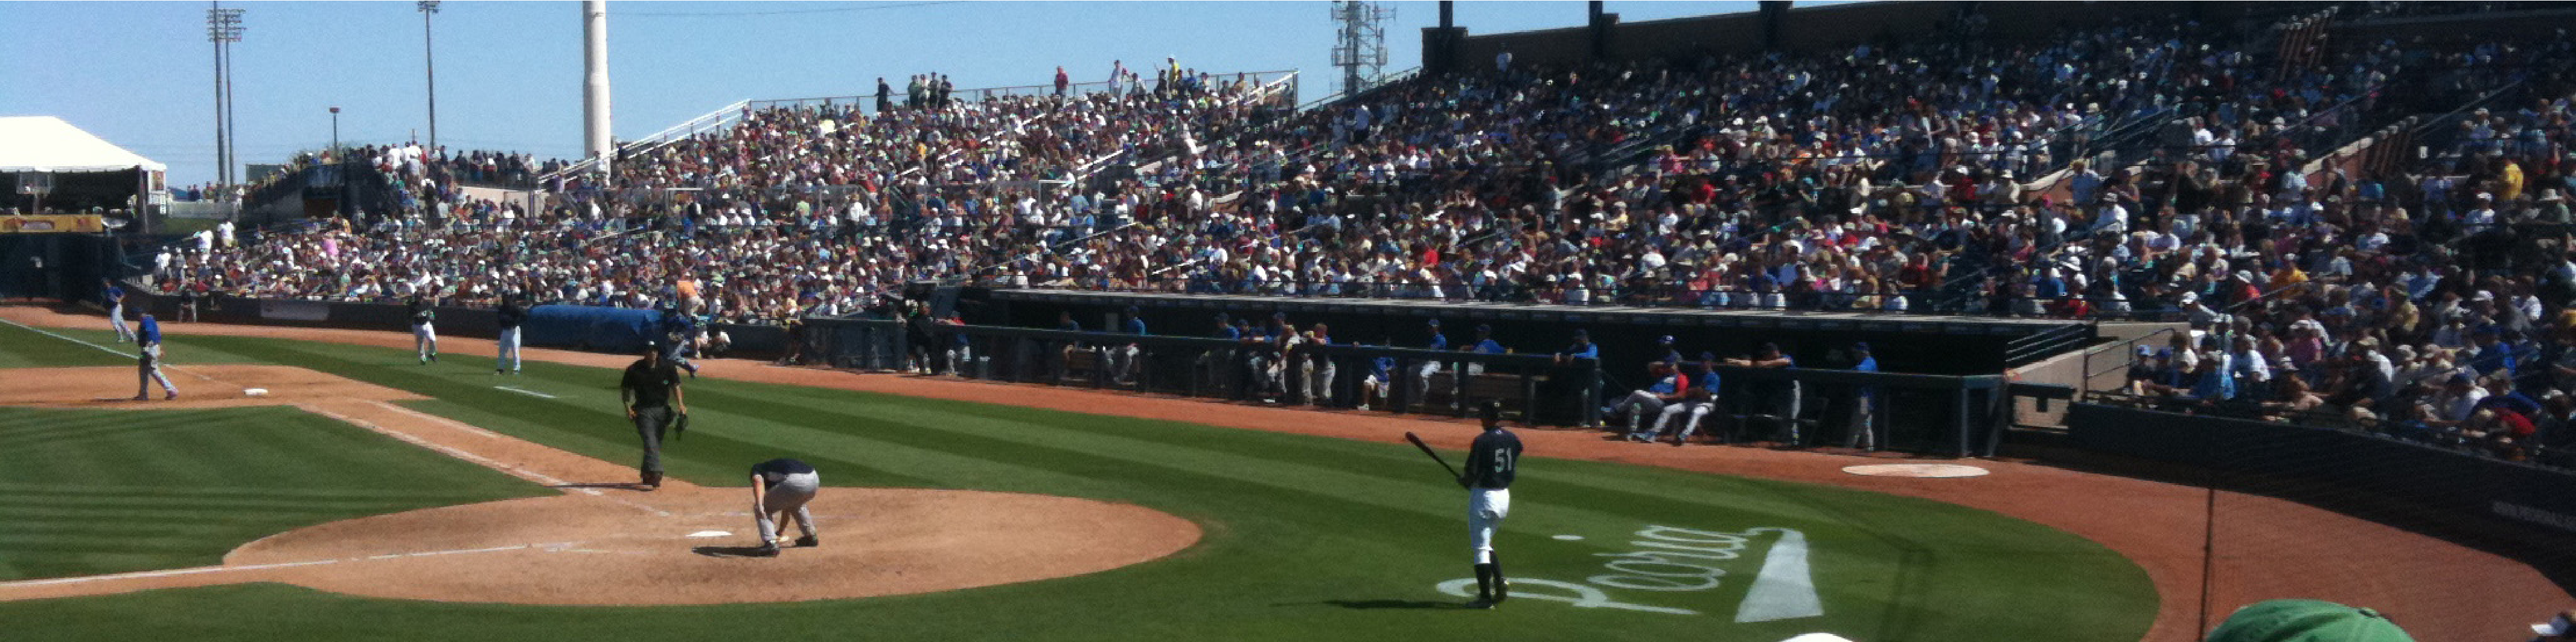
\includegraphics[width=\textwidth]{sampleteaser}
%  \caption{Seattle Mariners at Spring Training, 2010.}
%  \Description{Enjoying the baseball game from the third-base seats. Ichiro Suzuki %preparing to bat.}
%  \label{fig:teaser}
%\end{teaserfigure}

%
% This command processes the author and affiliation and title information and builds
% the first part of the formatted document.
\maketitle

\section{Introduction}

Learners of programming around the world who are writing, running, and debugging code in introductory programming courses (CS1) inevitably run into frustrating hurdles ~\cite{Drosos17}, including understanding programming\textquoteright \space basic concepts ~\cite{Mutka04,Garner05,Gomes15,Hristova03,Jenkins02,Milne02,Weintrop15}. Though people learn to program in different ways, such as with graphical programming blocks, text, or both  ~\cite{Weintrop15,Lee14,Ichinco17}, and for different reasons ~\cite{Bergstrom16}, few consider it an easy task ~\cite{Gomes15,Jenkins02, Lahtinen05}. This can be perceived through failure and dropout rates, which reach about 28\% among undergraduate students  ~\cite{Bennedsen07,Bosse16}.

Preparing new generations of professional and casual developers is a big challenge. If instructors are to overcome the difficulties students face, quell their frustrations, and help them achieve their goals, they need both knowledge of content and pedagogy ~\cite{Redish96,Shulman86,Shulman87}. Pedagogical knowledge includes three types of information: difficulties faced by students as they attempt to learn the content, typical paths students need to traverse to understand the content, and a set of strategies instructors can use in classes to avoid the difficulties ~\cite{Bransford00}. 

Our research was developed to help instructors of CS1 prepare their classes and improve their teaching strategies so they can support students learning to program in C or Python. For that, we focus on two research questions:

RQ1 - What are the difficulties students face when learning how to program?

RQ2 - What didactic strategies do instructors use to overcome these difficulties?

Experienced teachers acquire knowledge of content and pedagogy and know the types of difficulties students have and how to circumvent them  ~\cite{Bransford00}.  However, research has shown that expertise can lead to over-confidence in one\textquoteright s knowledge, meaning teachers can overlook details when teaching a topic they know well ~\cite{Fisher15}.  Even so, that knowledge can help other instructors in the task of how, for instance, to better organize the content for students ~\cite{Bransford00}. Taking  this into account, we collected qualitative data from two sources of data: semi-structured interviews with 16 professors from the University of Sao Paulo - USP - Brazil and diaries maintained by 110 students when taking CS1 at the same university. This data was analyzed using Grounded Theory techniques. The findings were reviewed by experienced instructors to confirm the results, in addition, it was collected the inexperienced instructors\textquoteright \space perspectives about the importance of this material. The main contribution of this paper is a set of difficulties faced by students learning programming, a classification of the most harmful challenges, and the didactic strategies usually used to teach and avoid them. This material can guide instructors, especially inexperienced ones, to prepare their classes, helping them improve their teaching and students\textquoteright \space learning.

\section{Related Work}

We organize our literature review according to the difficulties students face, and then the methods and strategies instructors use to teach the content. 

\textbf{Difficulties:} The content covered in programming courses can be difficult to understand, such as pointers and abstract data types ~\cite{Mhashi13,Piteira13}. According to Mhashi and Alakeel ~\cite{Mhashi13}, the most difficult programming concepts are repetition, recursion, lists, pointers, passing parameters, abstract data types, and the use of libraries. Some of these difficulties also appear in the research from Sevella and Lee ~\cite{Sevella13}. They further show that students confuse \textquoteleft For\textquoteright \space and \textquoteleft While\textquoteright \space concepts in C and find it difficult to use functions, sometimes developing programs without ever using this feature. In addition, they point out difficulties with variables: students forget to declare them or assign wrong types. They also note difficulties   with selection structures, such as writing conditional statements and nested selections. They found no difficulty with understanding lists. However, for the instructors responding to the questionnaire by Piteira and Costa ~\cite{Piteira13}, lists are among the most difficult topic, aside from pointers, structured data types, error handling, and parameters. Pointers and passing parameter by reference are also considered two of the most difficult topics by Lahtinen and colleagues ~\cite{Lahtinen05}. Piteira and Costa ~\cite{Piteira13} add that other difficulties for students include the use of language libraries and abstract data types. Regarding syntax, Hristova and colleagues ~\cite{Hristova03} report the wrong use of \textquoteleft =\textquoteright \space vs \textquoteleft==\textquoteright, \textquoteleft\&\&\textquoteright \space vs \textquoteleft\&\textquoteright, \textquoteleft \textbar\textbar\textquoteright \space vs \textquoteleft \textbar\textquoteright, different amounts of opening and closing parentheses, brackets and quotation marks, wrong separators in \textquoteleft For\textquoteright \space loops, and so on. 

\textbf{Methods and strategies used to teach basic programming content:} Traditional teaching methods can be inadequate for many students: teaching is not personalized, and dynamic concepts are presented with static material ~\cite{Gomes07}. 
In contrast, Deek and colleagues~\cite{Deek98} have developed an approach to programming courses that helps students learn concepts and their uses. In this approach, language characteristics were gradually introduced to students only in the context of specific problems. This has been shown to have positive effects on student achievement and confidence in programming. There are also programming tools that allow students to overcome the barriers to learning to program themselves ~\cite{Lee14, Ichinco17, Cao12}, and to give automatic feedback to students about their codes ~\cite{Ichinco14, Pino12}, not only feedback on syntax questions, but also on program semantic issues ~\cite{Repenning11}. Another approach for increasing students\textquoteright \space knowledge and developing their abilities is to increase the number of exercises, carefully selecting and solving them afterwards ~\cite{Mhashi13}. While visualization techniques to show complex concepts can help, visualizations are most often used for algorithm animation, with less emphasis on illustrating the basic structure of programs and their execution ~\cite{Mhashi13}.

While the literature tends to focus on the content students consider difficult, we seek to identify a set of difficulties students face in CS1 in order to organize a set of strategies that instructors may use to avoid them and improve learning.

\section{METHODOLOGY}

We conducted semi-structured interviews with 16 instructors and asked students to maintain diaries. Figure \ref{fig:Method} shows an overview of our methodology, which is detailed below.

\begin{figure}
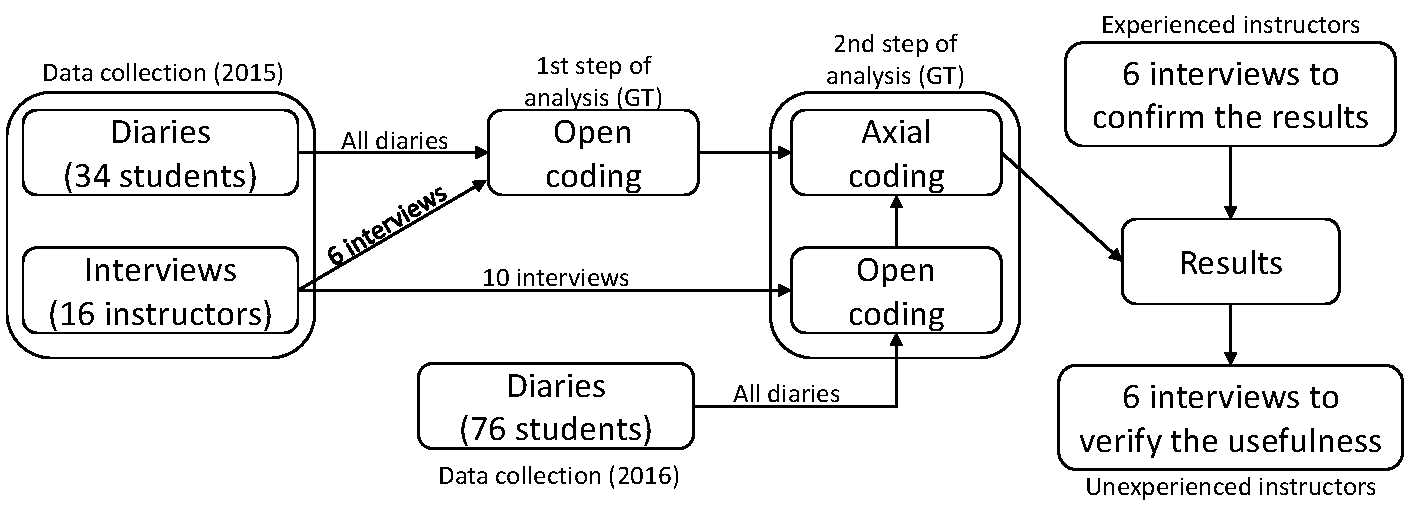
\includegraphics[height=1.5in, width=3.3in]{Methodology}
\caption{Scheme of the methodology.}
\label{fig:Method}
\end{figure}

\subsection{Data Collection}
This study is motivated by a previous study conducted at the University of Sao Paulo (Brazil) from 2010 to 2014, based on data from approximately 18,500 students from various majors who enrolled in 29 CS1 courses ~\cite{Bosse16}. The results showed that approximately 30\% of these registrations resulted in failures and dropouts, which corroborates results obtained by Bennedsen and Caspersen ~\cite{Bennedsen07}. 

In the present study, we chose to further investigate these courses and topic-related issues. We conducted interviews with instructors to delve into particulars, focusing on the topics to gain a perspective of the students\textquoteright \space learning experiences and instructors\textquoteright \space teaching experiences ~\cite{Creswell14}. Sixteen instructors from the Computer Science Department at the University of Sao Paulo were selected for interviews. About 30 instructors from the department had taught this course at least once. The first 6 instructors interviewed were those who were teaching introductory programming for the six classes whose students were keeping diaries about the difficulties in learning how to program. The other 10 were randomly selected. Each instructor was identified with an ID comprising a P, followed by a number from 1 to 16. Table \ref{tab:instructors} shows the level of experience and gender of the subjects.

\begin{table}
  \caption{Instructors\textquoteright \space data.}
  \label{tab:instructors}
  \begin{tabular}{ccc}
    \toprule
    Professor ID&Years of Experience&Gender\\
    \midrule
    P1 - P3 & More than 40 years & 1 F and 2 M \\
    P4 - P5 & 31 to 40 years & 2 M \\
    P6 - P7 & 21 to 30 years & 2 M \\
    P8 - P12 & 11 to 20 years & 2 F and 3 M \\
    P13 - P16 & 1 to 10 years & 4 M \\
  \bottomrule
\end{tabular}
\end{table}

The interviews began with a very general question: \textquoteleft In your view, what are the difficulties faced by students in CS1?\textquoteright \space The instructor was then guided to talk about the following introductory topics: variables; assignment command; input and output functions; arithmetic, relational (\textless, \textgreater, =, ...) and logical (and, or not) expressions; selection (if...else) and repetition structures (while, for, ...); string manipulation; uni- and multi-dimensional arrays; structured data; functions; and pointers. Most of the interviews took about half an hour, but some lasted for up to an hour.

We arranged for students to fill out diaries during their studies, keeping us informed about their difficulties as they emerged. We collected data from 6 different classes in 2015 (34 students) and another 6 in 2016 (76 students), yielding a total of 110 student diaries. The diaries were arranged in shared documents (Google Docs). We asked the students to include: code snippets, especially the wrong ones; how they fixed the errors; and the doubts they had about learning the topics. To clarify possible misunderstandings about the text written by the students, the researchers sometimes posed questions in the diaries. Each student was also identified with an ID, composed by an S, followed by a number from 1 to 110. Table \ref{tab:students} shows the total and percentage of students by age range and the number of times they attended the course before (TACB).

 \begin{table}
  \caption{Students\textquoteright \space  data.}
  \label{tab:students}
  \begin{tabular}{crr}
    \toprule
    Age&Total&\%\\
    \midrule
    Not informed &  1 &  1\% \\
    15 - 24      & 84 & 76\% \\
    25 - 34      & 17 & 15\% \\
    35 - 44      &  6 &  5\% \\
    45 - 54      &  1 &  1\% \\
    55 - 64      &  1 &  1\% \\
  	\bottomrule
  \end{tabular}
  \space \space \space \space \space
  \begin{tabular}{crr}
    \toprule
    TACB&Total& \% \\
    \midrule
    0 & 81 & 74\% \\
    1 & 17 & 15\% \\
    2 & 6 & 5\% \\
    3 & 4 & 4\% \\
    4 & 1 & 1\% \\
    5 & 1 & 1\% \\
  	\bottomrule
  \end{tabular}
\end{table}


\subsection{Data Analysis}
For the analysis of the data, we used Grounded Theory (GT) techniques, as described by Strauss and Corbin ~\cite{Strauss15}. During the analysis, concepts, categories, and subcategories emerged. According to Corbin and Strauss ~\cite{Strauss90}, \textquotedblleft the procedures of grounded theory are designed to develop a well-integrated set of concepts that provide a thorough theoretical explanation of social phenomena under study.\textquotedblright \space The groupings of these concepts into a higher degree of abstraction are called \textquotedblleft categories\textquotedblright \space ~\cite{Strauss15}. 

The data was read and analyzed, and relevant information was marked with a tag, thus characterizing a concept. Grouping these concepts, categories emerged. We primarily focused on two of them: \textquoteleft Difficulties with the Topics\textquoteright \space and \textquoteleft Didactic Strategies.\textquoteright \space After that, all text highlighted with codes was read again to identify difficulties, strategies, and connections among both. To confirm the results obtained with the data analysis, the results were presented to six experienced instructors to validate the findings. Then, six other instructors were interviewed, all inexperienced with the teaching of programming, in order to verify their opinions about the importance of the results for preparing their classes.

\section{Findings and Discussion}
In this section, we present the results obtained in two categories defined in the data analysis, Difficulties and Strategies, answering the two research questions that guided our study.

\textbf {\textit{RQ1 - What are the difficulties students face when learning how to program?}}

The difficulties presented below are divided by topics addressed in the courses, which are listed in the methodology section. Figure \ref{fig:Difficulties} presents the set of difficulties reported by instructors and students, which we classified in three levels. The first level comprises difficulties considered the most impactful to learning programming, which are marked with two stars. The intermediate level is marked with a star, and the last level has no marking. After each difficulty appears the number X of times they are cited by instructors \textquoteleft p\textquoteright \space and the number Y of times cited by students \textquoteleft s\textquoteright: XpYs. The 16 interviewed instructors commented mainly on C and Python; most of the difficulties listed in the diagram are related to the C language.

\begin{figure*}
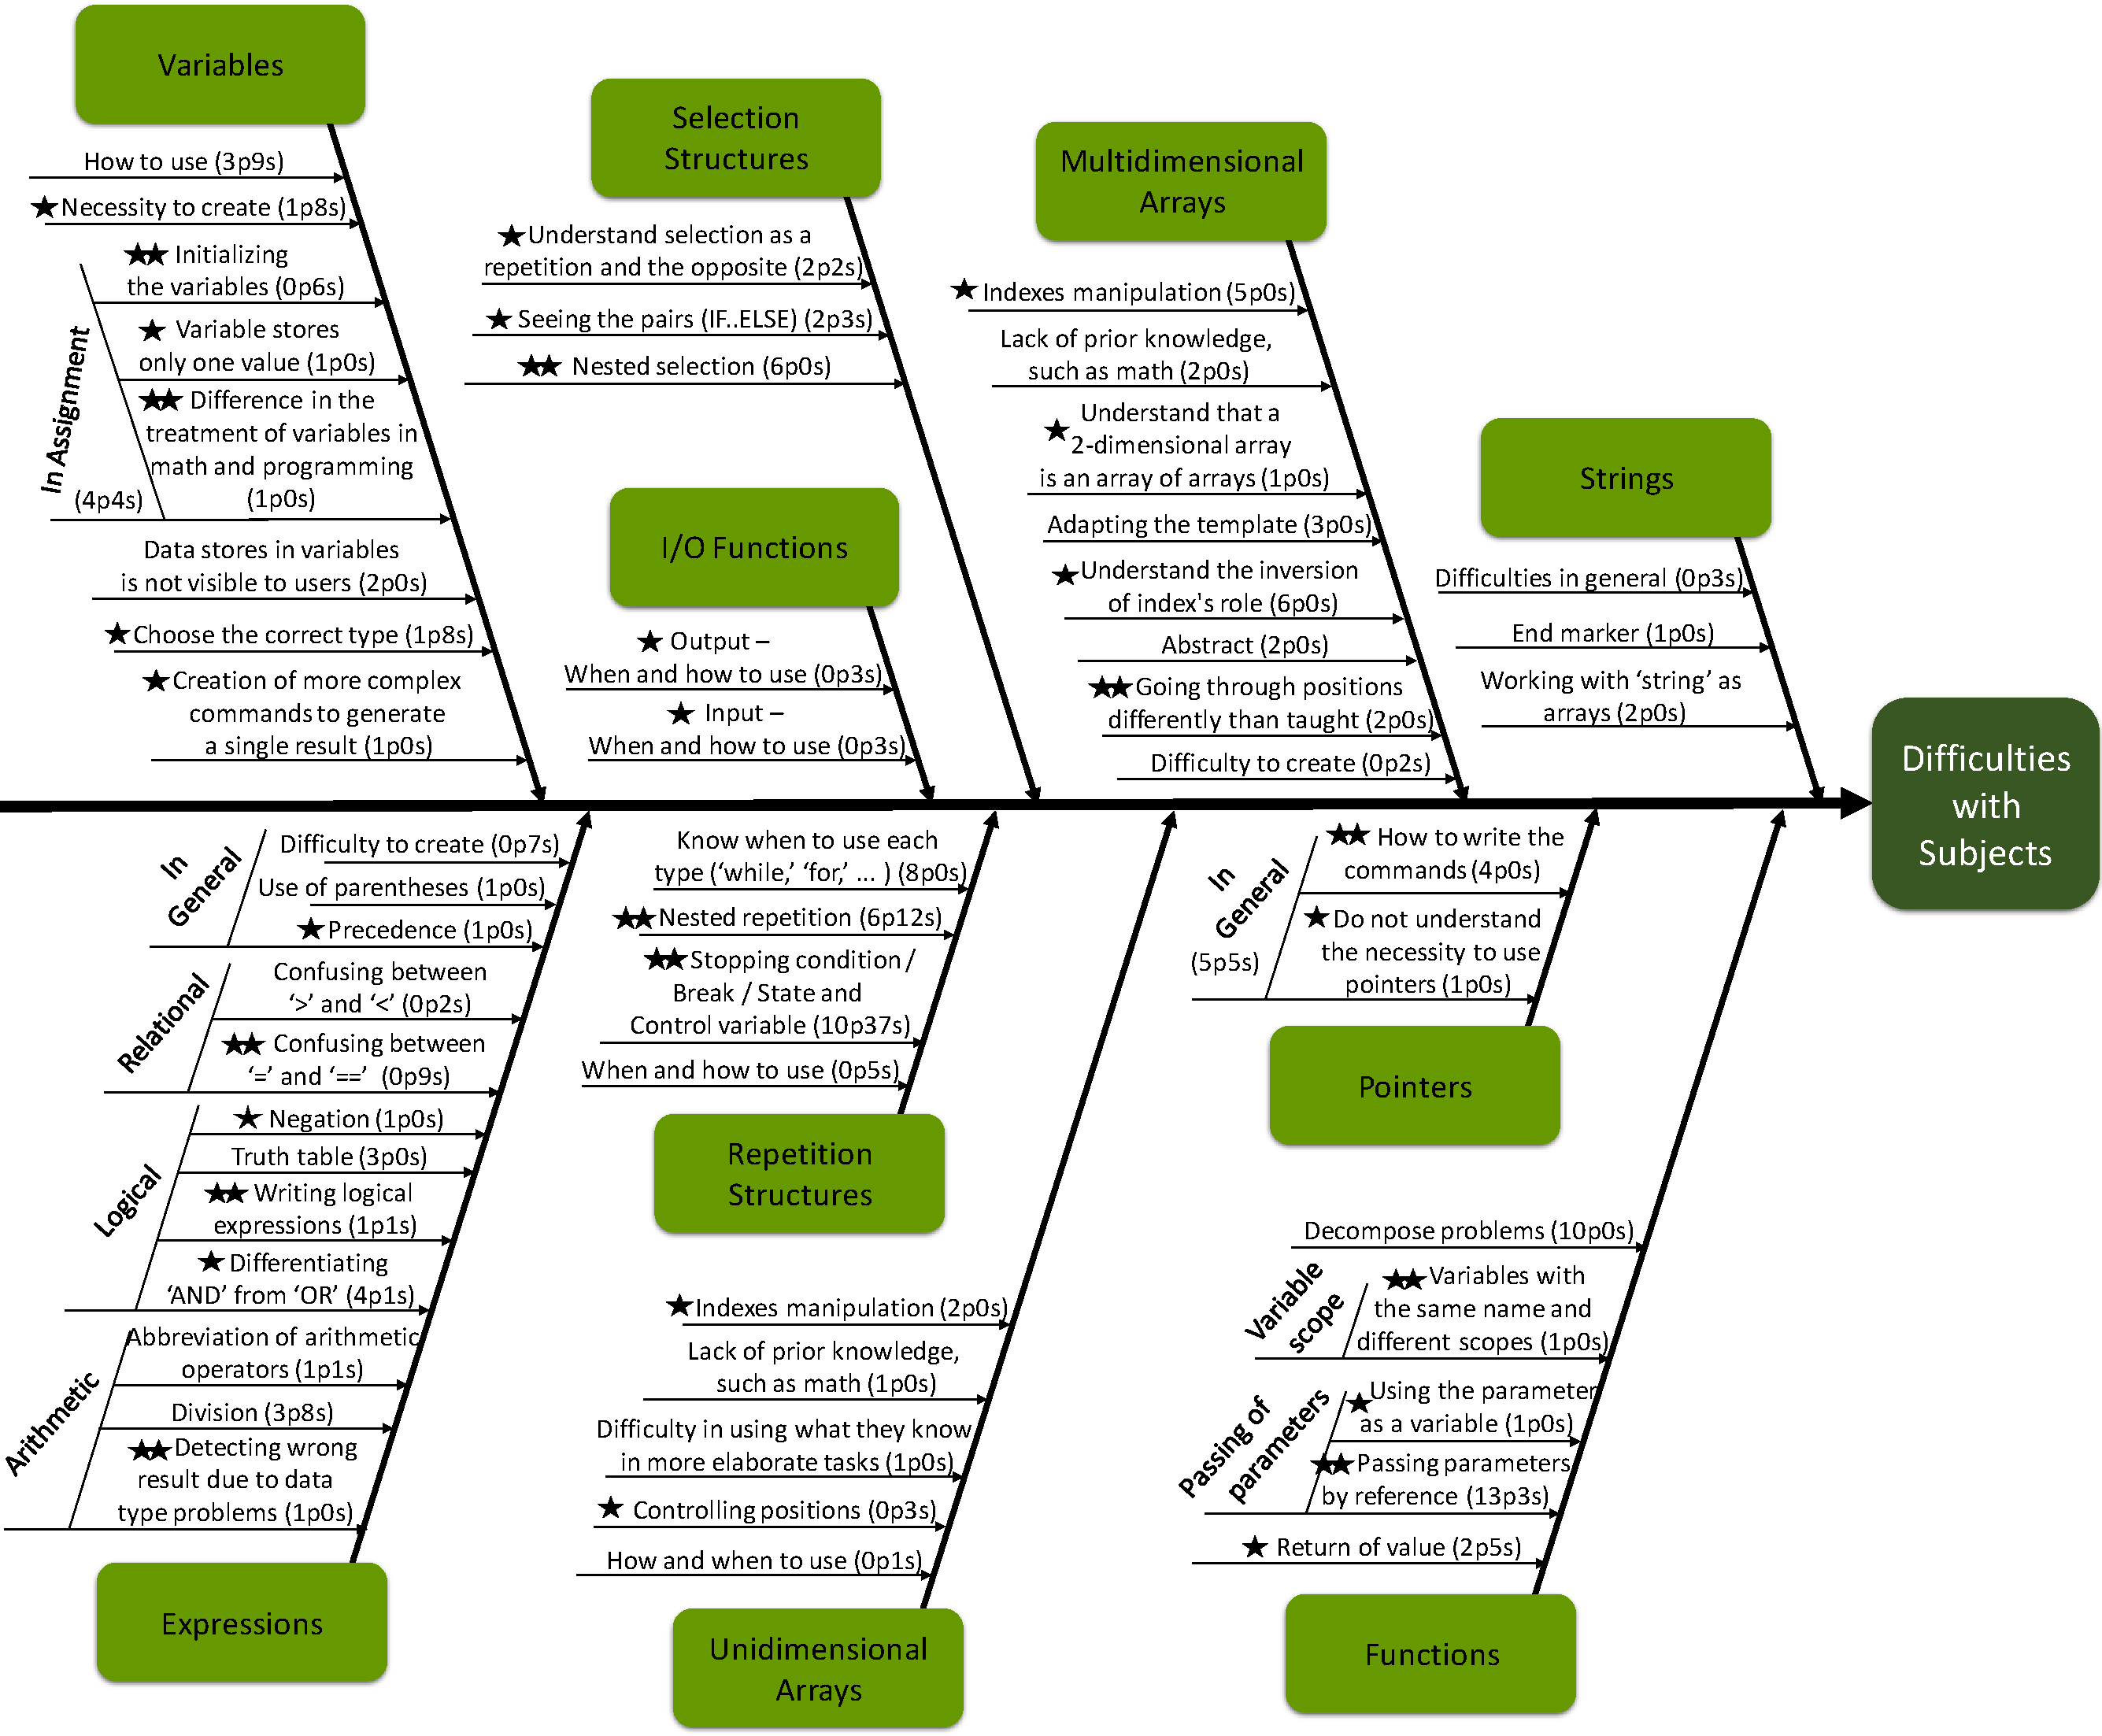
\includegraphics[height=6in, width=7in]{Difficulties1}
\caption{Diagram showing the list of difficulties per topics taught in introductory programming courses.}
\label{fig:Difficulties}
\end{figure*}

We found difficulties related to 10 topics taught in CS1, namely: Variables, Expressions, Input/Output Functions, Selection and Repetition Structures, Uni- and Multidimensional Array, Function, Pointer, and String. One of the difficulties of the first level of classification is \textbf{initializing the variables}, as shown in the topic \underline{Variable} of the diagram. Many students do not know if it is necessary to initialize and with what value: \textquotedblleft \textit{When compiling everything was fine, however, the final result (max) has a gigantic number ... problem tidy, I had not put the initial value of the variable max...}\textquotedblright \space - S18. In addition, the \textbf{difference in the treatment of variables in mathematics and programming} can generate doubt, as explained by P8: \textquotedblleft \textit{Then there are \textquoteleft{x = x + 1}\textquoteright \space and these students experiencing difficulty do not understand if you read as in math, \textquoteleft{x is equal to x + 1,}\textquoteright \space (student replies) that \textquoteleft{it is impossible for x to be equal to x + 1}\textquoteright.}\textquotedblright

Working with \underline{Expressions}, the result shows difficulties related to \textbf{detecting the wrong result due to data type problems}: \textquotedblleft \textit{... when it is a numerical operation, it is difficult for them to perceive the error. So, for example, an algorithm to calculate, make an average, ... yields zero (as a result) and sometimes the student realizes that they used integer rather than float}\textquotedblright \space - P7. Another source of difficulty is \textbf{writing logical expressions}. According to P11, \textquotedblleft \textit{...something that exists in natural language and that normally does not exist in programming language is something like \textquoteleft{x > 3 and < 5}\textquoteright \space and in computing I cannot write like this, you have to write \textquoteleft{x > 3 and x < 5}\textquoteright, then they write it wrong, they write \textquoteleft{x > 3 and < 5}\textquoteright.}\textquotedblright \space The students find it difficult to write logical expressions in the syntax of the programming language, which is usually different from that used in mathematics and natural language. And, as already cited by Hristova and colleagues ~\cite{Hristova03}, there is \textbf{confusion between \textquoteleft{=}\textquoteright \space and \textquoteleft{==}\textquoteright}. According to S34, this is a constant error: \textquotedblleft \textit{I wrote the program and noticed some difficulties I constantly face such as ... whether to use = or == within the Selections or Repetition Structures.}\textquotedblright

Regarding \underline{Selection Structures}, the most complicated task is working with \textbf{nested selections} with a set of pairs \textquoteleft{IF..ELSE}\textquoteright: \textquotedblleft \textit{When I had nesting, one selection within another, that caused a lot of confusion}\textquotedblright \space - P15. 
Similarly, the most complicated \underline{Repetition Structure} to learn is the creation and use of \textbf{nested repetition} structures, that is, two or more structures of repetition, with one inside the other. A classic example of using nested repetitions is the manipulation of multidimensional arrays. Other difficulties include the creation of the \textbf{stopping condition} and manipulating the \textbf{control variable}. According to P15, students begin to use the control variable without even initializing it, \textquotedblleft \textit{... they use a variable in the stop condition before assigning an initial value to this variable,}\textquotedblright \space and then they misuse the increment or decrement operators so that it satisfies the desired stop condition: \textquotedblleft \textit{... their challenge to generate a repetition structure was to understand the concept of a stop condition, how to create a stop condition, and how to make an increment of a variable that satisfies this condition.}\textquotedblright \space Manipulating variables is also a task necessary for working with \underline{Multidimensional Arrays}, where \textbf{going through positions differently than taught} is a source of difficulty, as exemplified by P14: \textquotedblleft \textit{... if we use a 2-dimensional array, for example, to represent a game board and ask to move diagonally, or backward, ... then things start to get confusing. Especially if the \textquoteleft{i}\textquoteright \space and \textquoteleft{j}\textquoteright \space (variables used to indicate the position in the row and column) that are there, begin to appear in a switched order.}\textquotedblright

Finally, for P4, when teaching \underline{Pointers}, \textquotedblleft \textit{the trouble starts to get bigger.}\textquotedblright \space Pointers are cited by many researchers as one of the most difficult topics ~\cite{Mhashi13,Piteira13,Sevella13}, and the results of this study confirmed this, as can be observed in the comment made by P14: \textquotedblleft \textit{But of the content of the course, I think the most difficult thing was for them to understand pointers.}\textquotedblright \space P13 reports that the students \textquotedblleft \textit{end up learning by heart,}\textquotedblright \space and adds \textquotedblleft \textit{I think they can understand, closer to the end of the second semester,}\textquotedblright \space that is, only in the subsequent course. Many even avoid teaching pointers: \textquotedblleft \textit{We try to avoid talking about pointers too}\textquotedblright \space - P10. Others end up showing them only because they are necessary to pass parameters by reference, and the main difficulty is \textbf{how to write the commands} using pointers. Working with \underline{Functions}, besides the difficulty with \textbf{passing parameters by reference}, students confuse \textbf{variables with the same name and different scopes}. 

\textbf { \textit{RQ2 - What didactic strategies do instructors use to overcome these difficulties?}}

During the interviews, instructors mentioned many strategies they used to teach the topics and to mitigate difficulties students face. In this paper, we present the strategies mentioned 5 times or more in the interviews. The third column of Table \ref{tab:Strategies} reports the topics or difficulties linked to the strategies. If the term General is used in this column, this means that this strategy was quoted at least once in each of the topics covered.

\begin{table}
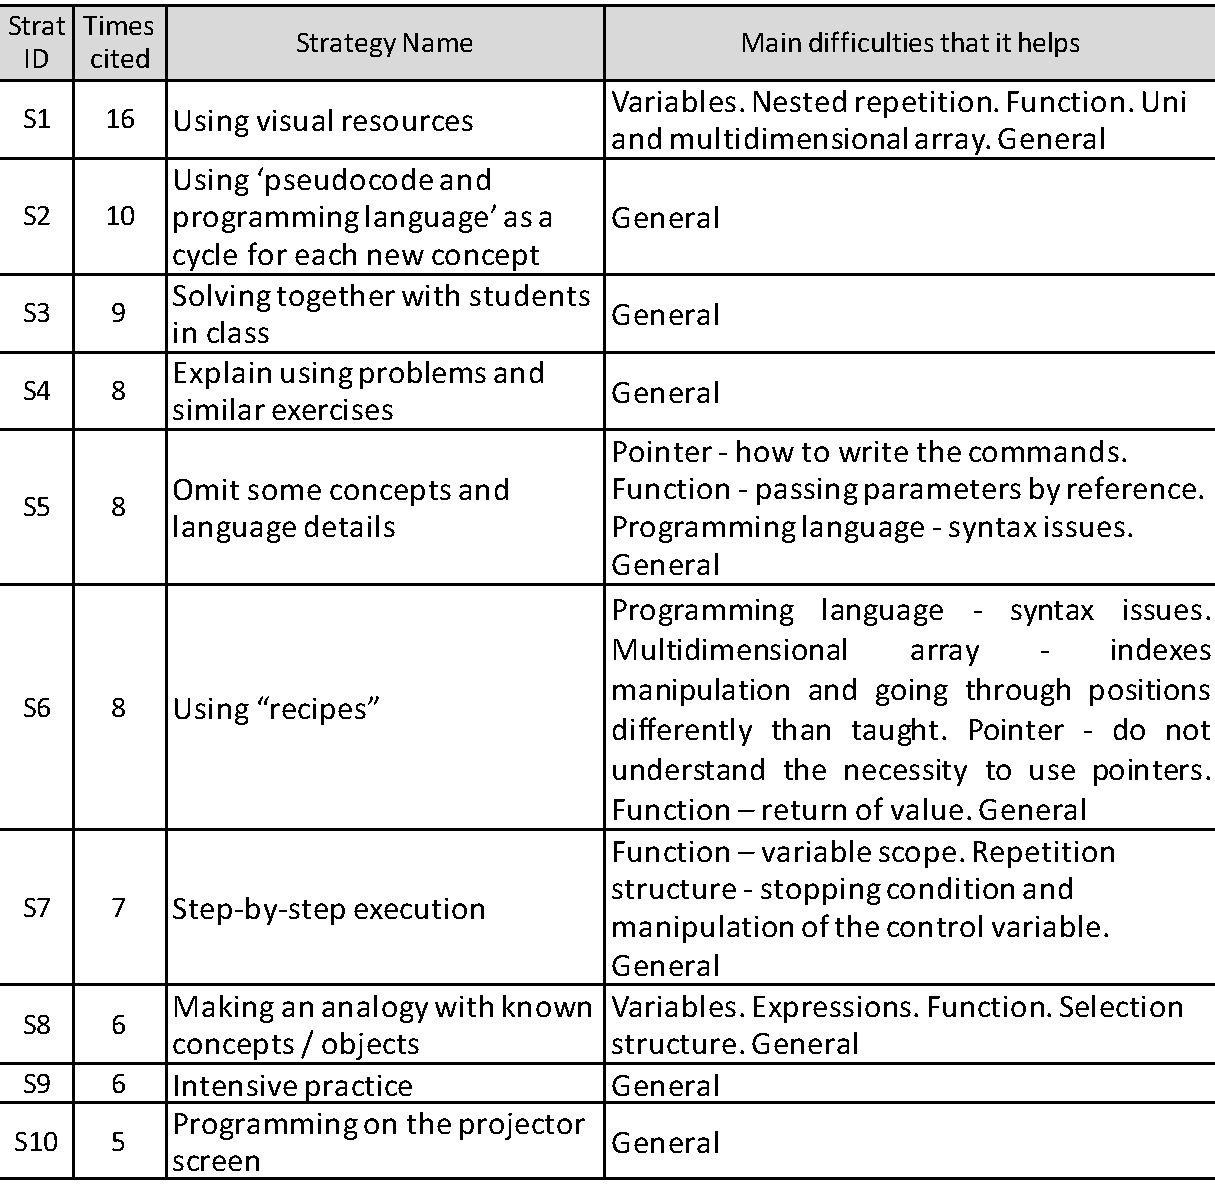
\includegraphics[height=3.8in, width=3.3in]{Strategies1}
  \caption{Strategy used to avoid or minimize the difficulties faced by students to learn how to program.}
  \label{tab:Strategies}
\end{table}

\textbf{Using visual resources (S1)}. Abstraction is one of the major problems of the course. It is difficult for the novice student to visualize where the data is, how it is processed, or how the commands work: \textquotedblleft \textit{...there is a difficulty in working with abstract concepts...}\textquotedblright \space - P9 and P15 remembered \textquotedblleft \textit{...classes that at first did not work, you had to have something visual too}\textquotedblright \space and cited an example \textquotedblleft \textit{Variable declaration needs to be visual ... explaining that declaring a variable will occupy space in memory, this abstraction is a bit difficult.}\textquotedblright \space The \textquoteleft{visuals}\textquoteright can be drawings: \textquotedblleft \textit{...I draw the memory...}\textquotedblright \space - P9 or made using features like arrows that represent the input and output of the data in a function, for example: \textquotedblleft \textit{I always do in a graphic way the inputs and outputs, with arrows}\textquotedblright \space - P8. Another form of visual presentation is \textquotedblleft \textit{...animations, if I needed to show that visually...}\textquotedblright \space - P15 and adds that \textquotedblleft \textit{...there are many visual resources on the internet....}\textquotedblright

\textbf{Using \textquoteleft{pseudocode and programming language}\textquoteright \space as a cycle for each new concept (S2)}. Few instructors begin the course with pseudocode before progressing to a programming language, \textquotedblleft \textit{With the algorithm in pseudo-language, I did not see much success ... having two simultaneous languages was not going to be as effective}\textquotedblright \space - P16. Most of the interviewed instructors use pseudocode only to teach the concept and then immediately show the same concept in the programming language: \textquotedblleft \textit{... I give the algorithmic concept and after this, I go to the program ... I do it like this, coming and going}\textquotedblright \space - P9. According to P11, \textquotedblleft \textit{The programming language is a tool to teach algorithms and data structures}\textquotedblright \space and the pseudocode or pseudo language is quickly used, without many rules, only to explain the concepts.

\textbf{Solving together with students in class (S3)}. This is another highly used strategy: to \textquotedblleft \textit{solve and write problems together with the students ... the idea is to let them participate and they try to develop the program together. Often times, I show the program even knowing that it is wrong and we try to find (the mistake)}\textquotedblright \space - P3. Many instructors reported using this strategy and claim it works because students participate and can see step-by-step how the program is developed.

\textbf{Explain using problems and similar exercises (S4)}. To introduce and show the usefulness of the concepts that need to be taught in the course, one strategy is to use problems: \textquotedblleft \textit{I usually start explaining a content by describing a problem}\textquotedblright \space - P16. For P10, it is a way to motivate students, \textquotedblleft \textit{...we try to motivate by using some problems,}\textquotedblright \space because the student sees the concept\textquoteright s usefulness in practice and learns how it should be used. Between presenting the first problem to the student and more complex exercises, P16 advises \textquotedblleft \textit{...also bring to class exercises that are similar but do not solve exactly that problem.}\textquotedblright \space In this way, the student can practice what was taught, and then use it in other situations.

\textbf{Omit some concepts and language details (S5)}. Details of the coding language can hinder the development of the code. If the instructor omits some details, they may improve initial learning: \textquotedblleft \textit{The idea was to abstract the language syntax somewhat}\textquotedblright \space - P15. P5 also said \textquotedblleft \textit{...if I have to teach in C, I do not explain an input command. I even joke: \textquoteleft{Look, God told you to do it like this.}\textquoteright},\textquotedblright \space because if you explain every detail of the syntax, the content does progress. Concepts are also omitted at times when they are not indispensable. An example of this was offered by P1, with the following statement:  \textquotedblleft \textit{Passing parameter is also all by pointer, I do not need to speak of pointers, they do the exercise without problems ... they are hidden from them, these concepts, but they are in fact using (them).}\textquotedblright

\textbf{Using \textquotedblleft{recipes}\textquotedblright \space (S6)}. In content that is considered more complicated, as is the case of passing parameters by reference using pointers,: \textquotedblleft \textit{When we teach with C we make the passage by reference, but we provide a \textquoteleft{recipe}\textquoteright, so it is (I use) \textquoteleft{\&}\textquoteright \space when I call the function and within the function \textquoteleft{*}\textquoteright . }\textquotedblright \space - P12. In addition, to avoid language syntax explanations often unnecessary for the moment, such as \textquoteleft{scanf}\textquoteright \space and \textquoteleft{printf}\textquoteright \space in the C programming language, instructors use a kind of \textquoteleft{recipe;}\textquoteright \space that is, a step-by-step instruction of how something should be done.

\textbf{Step-by-step execution (S7)}. Another frequently used technique is step-by-step execution, so that the student sees what is happening in the program, which also helps them find existing errors in the code. This execution is done on the board or even using the projector. Everything that happens, from change of values in the variables to the output of a repetition or change of variable scope, is line-by-line shown and analyzed during this exercise: \textquotedblleft \textit{I used slides that were showing repetition actually happening as a debugging of the program and going through each instruction line}\textquotedblright \space - P15. However, for more advanced students, this exercise can be a bit tedious.

\textbf{Making an analogy with known concepts / objects (S8)}. This involves using an everyday example from the real world, with situations familiar to the student, as P3 suggested: \textquotedblleft \textit{make an association with a real-world problem where you have the same type of separation (situation). I think this makes sense, so it helps a lot.}\textquotedblright \space In reference to arithmetic, logical, and relational expressions, P1 said that \textquotedblleft \textit{they (the students) confuse a lot... I started with day to day examples}\textquotedblright \space and P11 reinforces that \textquotedblleft \textit{I think this is a fundamental thing, exercises that have to do with the universe of the student.}\textquotedblright \space

\textbf{Intensive practice (S9)}. Five instructors cited intensive practice during the interviews, corroborating results presented by Mhashi and Alakeel ~\cite{Mhashi13}. According to P13, \textquotedblleft \textit{The student has to arrive, sit, study, work, exercise and solve as many exercises as possible. It is very Kumon style. It is training, training, training.}\textquotedblright \space Feedback is also important, as P11 said \textquotedblleft \textit{I give a lot of exercises for them to do in the classroom, from there they do on paper..., if we have three solutions (made by students in the classroom), I ask the 3 students to go (to write on the board) and I show the three different solutions. Then we discuss the 3 solutions.}\textquotedblright \space 

\textbf{Programming on the projector screen (S10)}. Lastly, this strategy includes developing the code during class, projecting it so that the student can see and participate, and collaboratively making changes and showing the results: \textquotedblleft \textit{I use blackboard and projector ... writing a program in the act and running it}\textquotedblright \space - P15 and P14 said that this \textquotedblleft \textit{...makes a significant difference.}\textquotedblright \space

In addition, future confirmatory research could yield data beyond instructors\textquoteright \space experiences, exploring the degree of student development in the CS1 courses that use those strategies.  Linking the findings to existing pedagogical theories could be of great value to add knowledge and increase the contribution of these results. 
\section{Validation of the Results}
After compiling the results, they were validated by 6 experienced instructors. Each of them was asked about the difficulties listed by topic and didactic strategies mentioned. During these interviews, one new idea arose: a suggestion to classify the difficulties as explained in the Findings section. Having confirmed our findings, six inexperienced instructors (Pu) were interviewed. These instructors had taught less than three CS1 courses and work in universities of different states in Brazil. We asked them to comment on the importance of this information about difficulties and strategies. The difficulties were showed to them without the classification presented in this paper. Even unaware of this suggestion given by experienced instructors, two of them commented on the importance of classification, as indicated in a comment made by Pu4:  \textquotedblleft \textit{...the list of difficulties could help me to organize my classes, but I think that if the difficulties had a classification, showing which of them are the most harmful for students learning programming, it could be easier to use in practice...}\textquotedblright 

All of the six inexperienced interviewed instructors said that the list of difficulties and strategies could greatly help to plan the material used with students and in explaining the topics, as commented by Pu6: \textquotedblleft \textit{...knowing the difficulties, I would work out the topic in the classroom so that the difficulty arise and so I would help them solve the doubts...}\textquotedblright \space Three of them commented that most of the difficulties could be minimized or eliminated depending on the programming language used, citing Python as an example. They added that the difficulties exist not only for C language, but also for many others, like Java. One important point they addressed regarded the topics and/or difficulties linked to the strategies.  Even though most strategies are known , this connection could help to determine the best strategy at certain times in class.

\subsection{Threats to Validity}
The data was collected from experienced instructors from the same department who teach in different colleges at a single university. This factor may raise some doubts as to the accuracy of the results in other contexts. A survey could be created to confirm the results obtained and to complete the set of difficulties and didactic strategies. 

\section{Conclusion}
Learning to program is not an easy task ~\cite{Lahtinen05}. Students who study programming face many difficulties, as do their instructors. Some difficulties related to content are generally mild; they can be quickly clarified with examples of application and practical exercises, as is the case in understanding variables. Other difficulties are more complicated, requiring instructors to use several resources to improve learning and not always successfully. One such case is the topic Pointer. Many instructors shared their desire to avoid this topic in CS1, because they consider it too difficult. However, it is necessary for teaching other content, such as pass parameters by reference in C, in the topic Function. Pointer concepts are often omitted (S4) and/or used in the form of \textquoteleft{recipes}\textquoteright \space (S8), so there is no need to delve deeper into them in CS1. In addition, functions, uni- and multi-dimensional arrays, and repetition structures (while, for, ...) are considered the three most difficult topics in the instructors' view.

To teach CS1, inexperienced instructors consider it useful to have the list of difficulties students face and the strategies they can use to teach the content and avoid them. According to them, having knowledge of the difficulties could change the way they teach; for example, they can choose exercises that make the difficulties arise during the class, so that they can support students in solving them. About the strategies, we received good feedback from inexperienced instructors as well. Although many of them were already aware of many of the strategies on the list, they considered it important to have the list, in part because some of the strategies were linked to the difficulties that could be avoided, and also because the list tends to make them remember each one, making it easier to integrate them into a class. The contribution of our paper may improve pedagogical knowledge to better teach and consequently better learn programming.

%
% The acknowledgments section is defined using the "acks" environment (and NOT an unnumbered section). This ensures
% the proper identification of the section in the article metadata, and the consistent spelling of the heading.
\begin{acks}
  We thank the instructors and students who kindly provided us with the data that made this study possible. We also thanks to CAPES, this study was financed in part by the \textquotedblleft {Coordenacao de Aperfeicoamento de Pessoal de Nivel Superior} \textquotedblright \space - Brazil (CAPES) - Finance Code 001.
\end{acks}

%
% The next two lines define the bibliography style to be used, and the bibliography file.
\bibliographystyle{ACM-Reference-Format}
\bibliography{sample-base}

\end{document}
